\chapter{Sequenzdiagramme}
Um die verschiedenen möglichen Abläufe zu verdeutlichen wurden einige Sequenzdiagramme erstellt, die die Funktionen der Anwendung einfach und effektiv zu erklären.



\begin{itemize}

    \item 
    
    \begin{figure}[h]
      \centering
      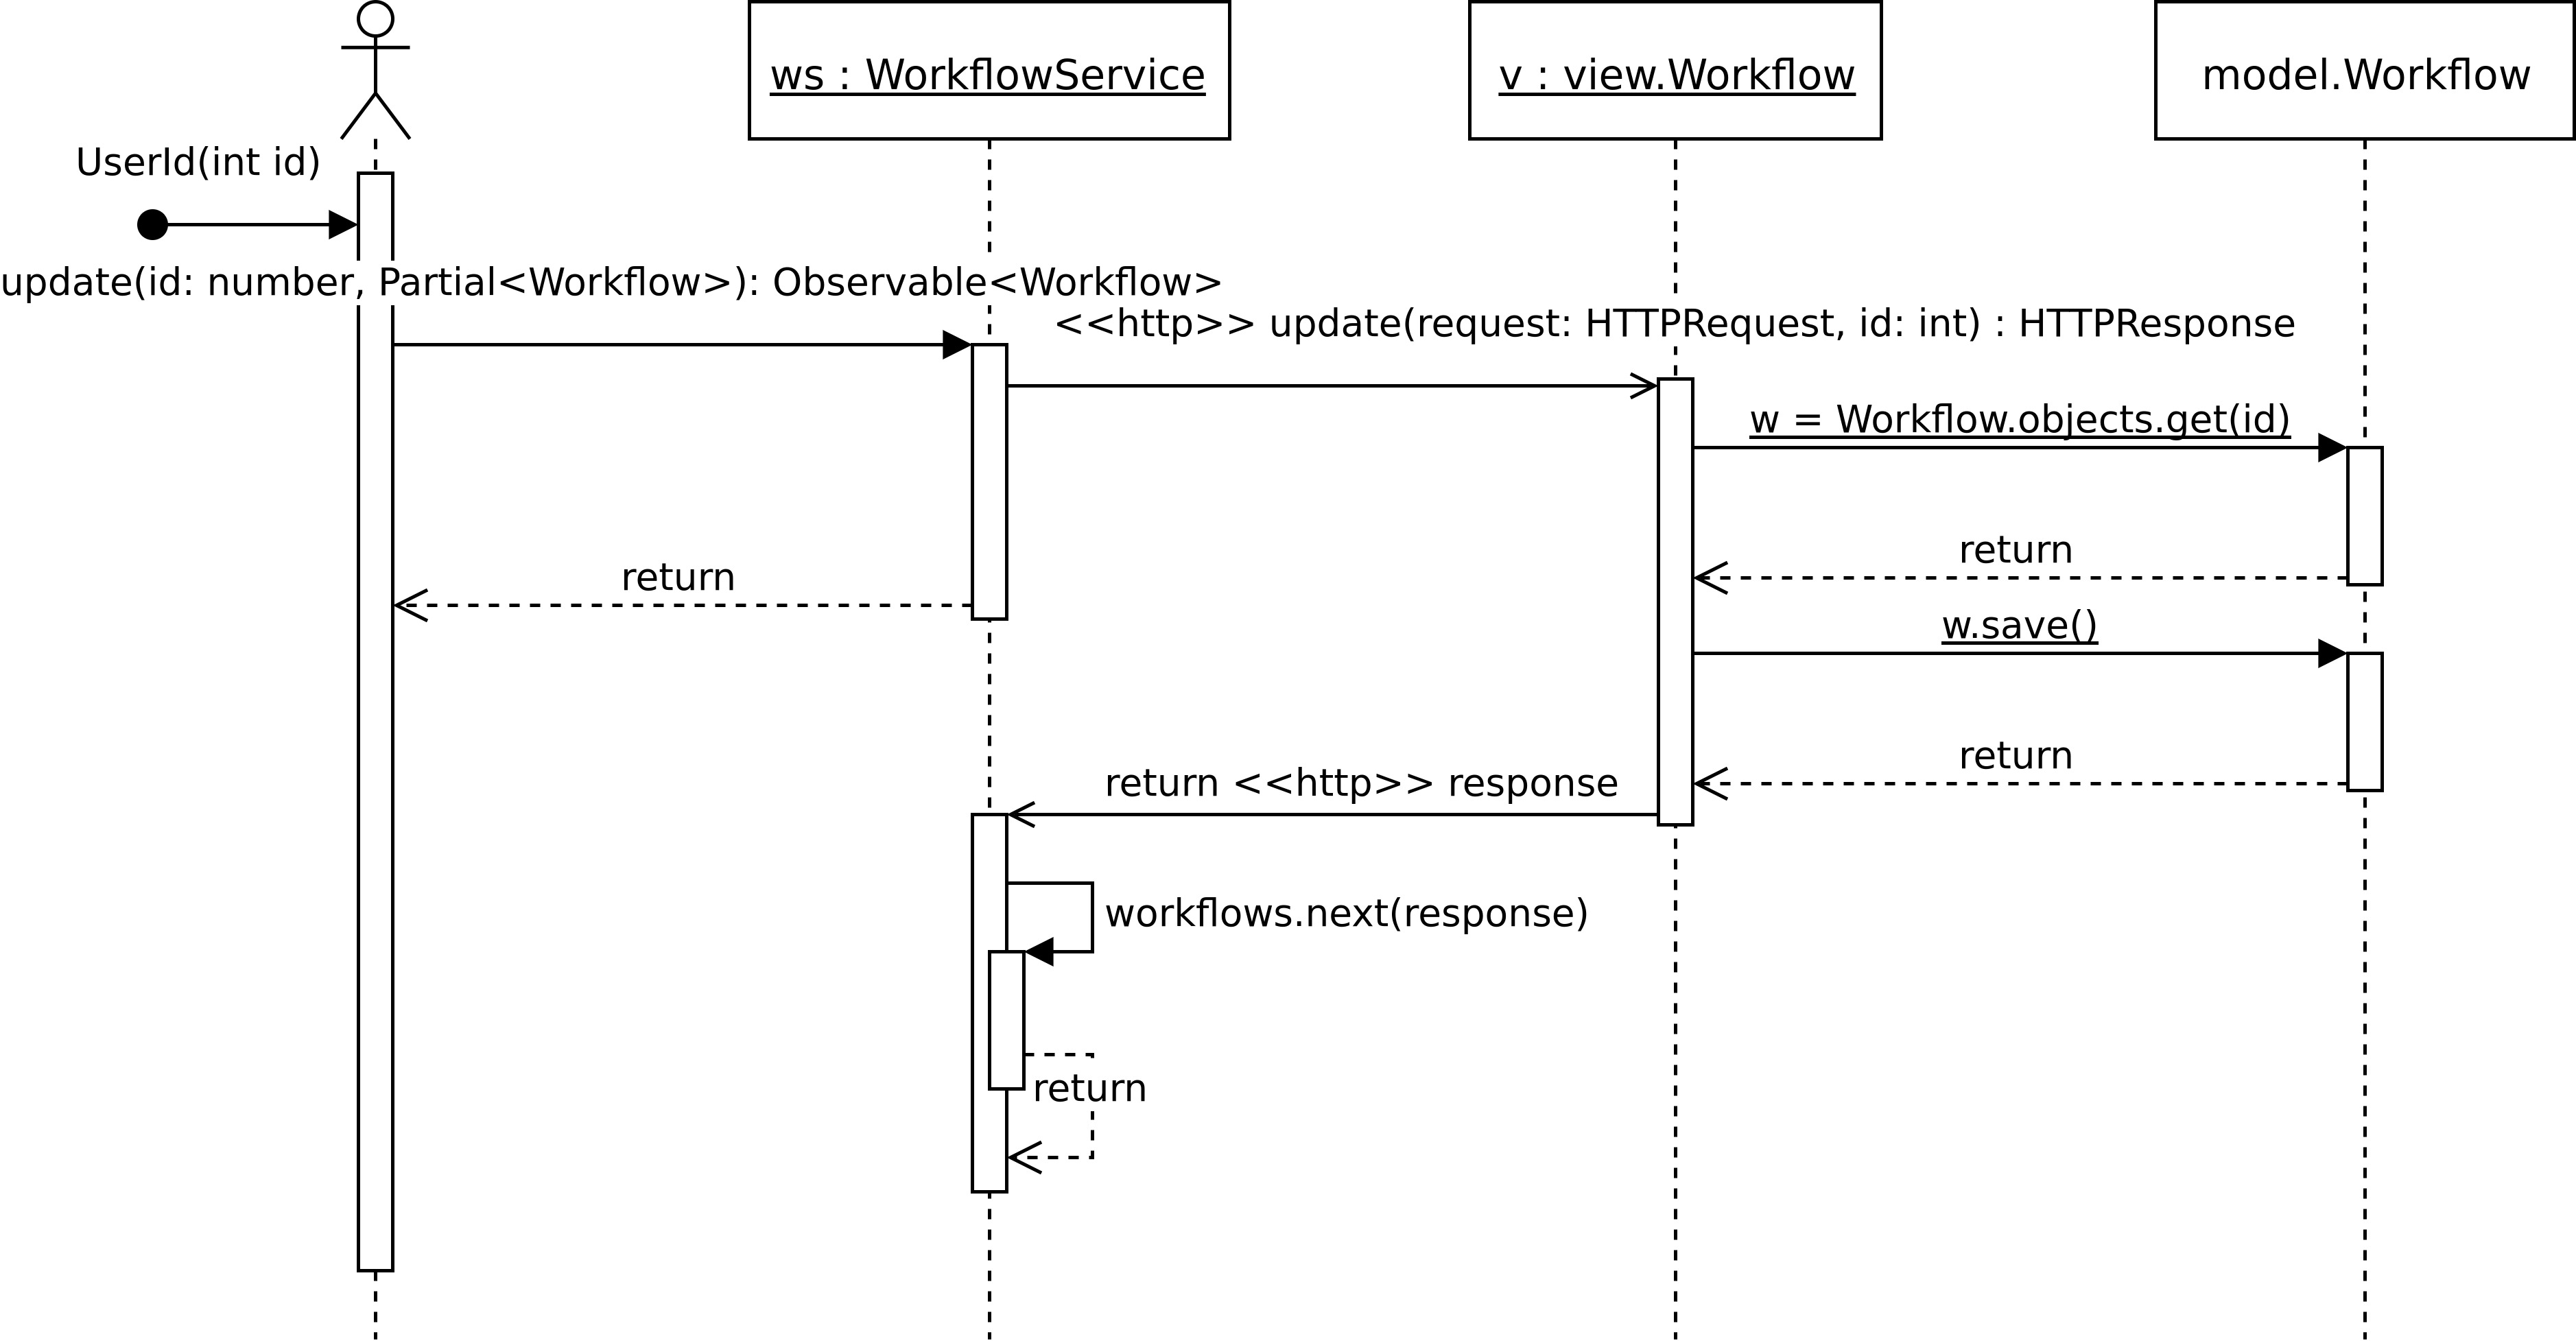
\includegraphics[width=15cm]{images/sqd_edit_workflow.jpg}
      \caption{caption}
      \label{fig:sqd_edit}
    \end{figure}
    
    \begin{figure}[h]
      \centering
      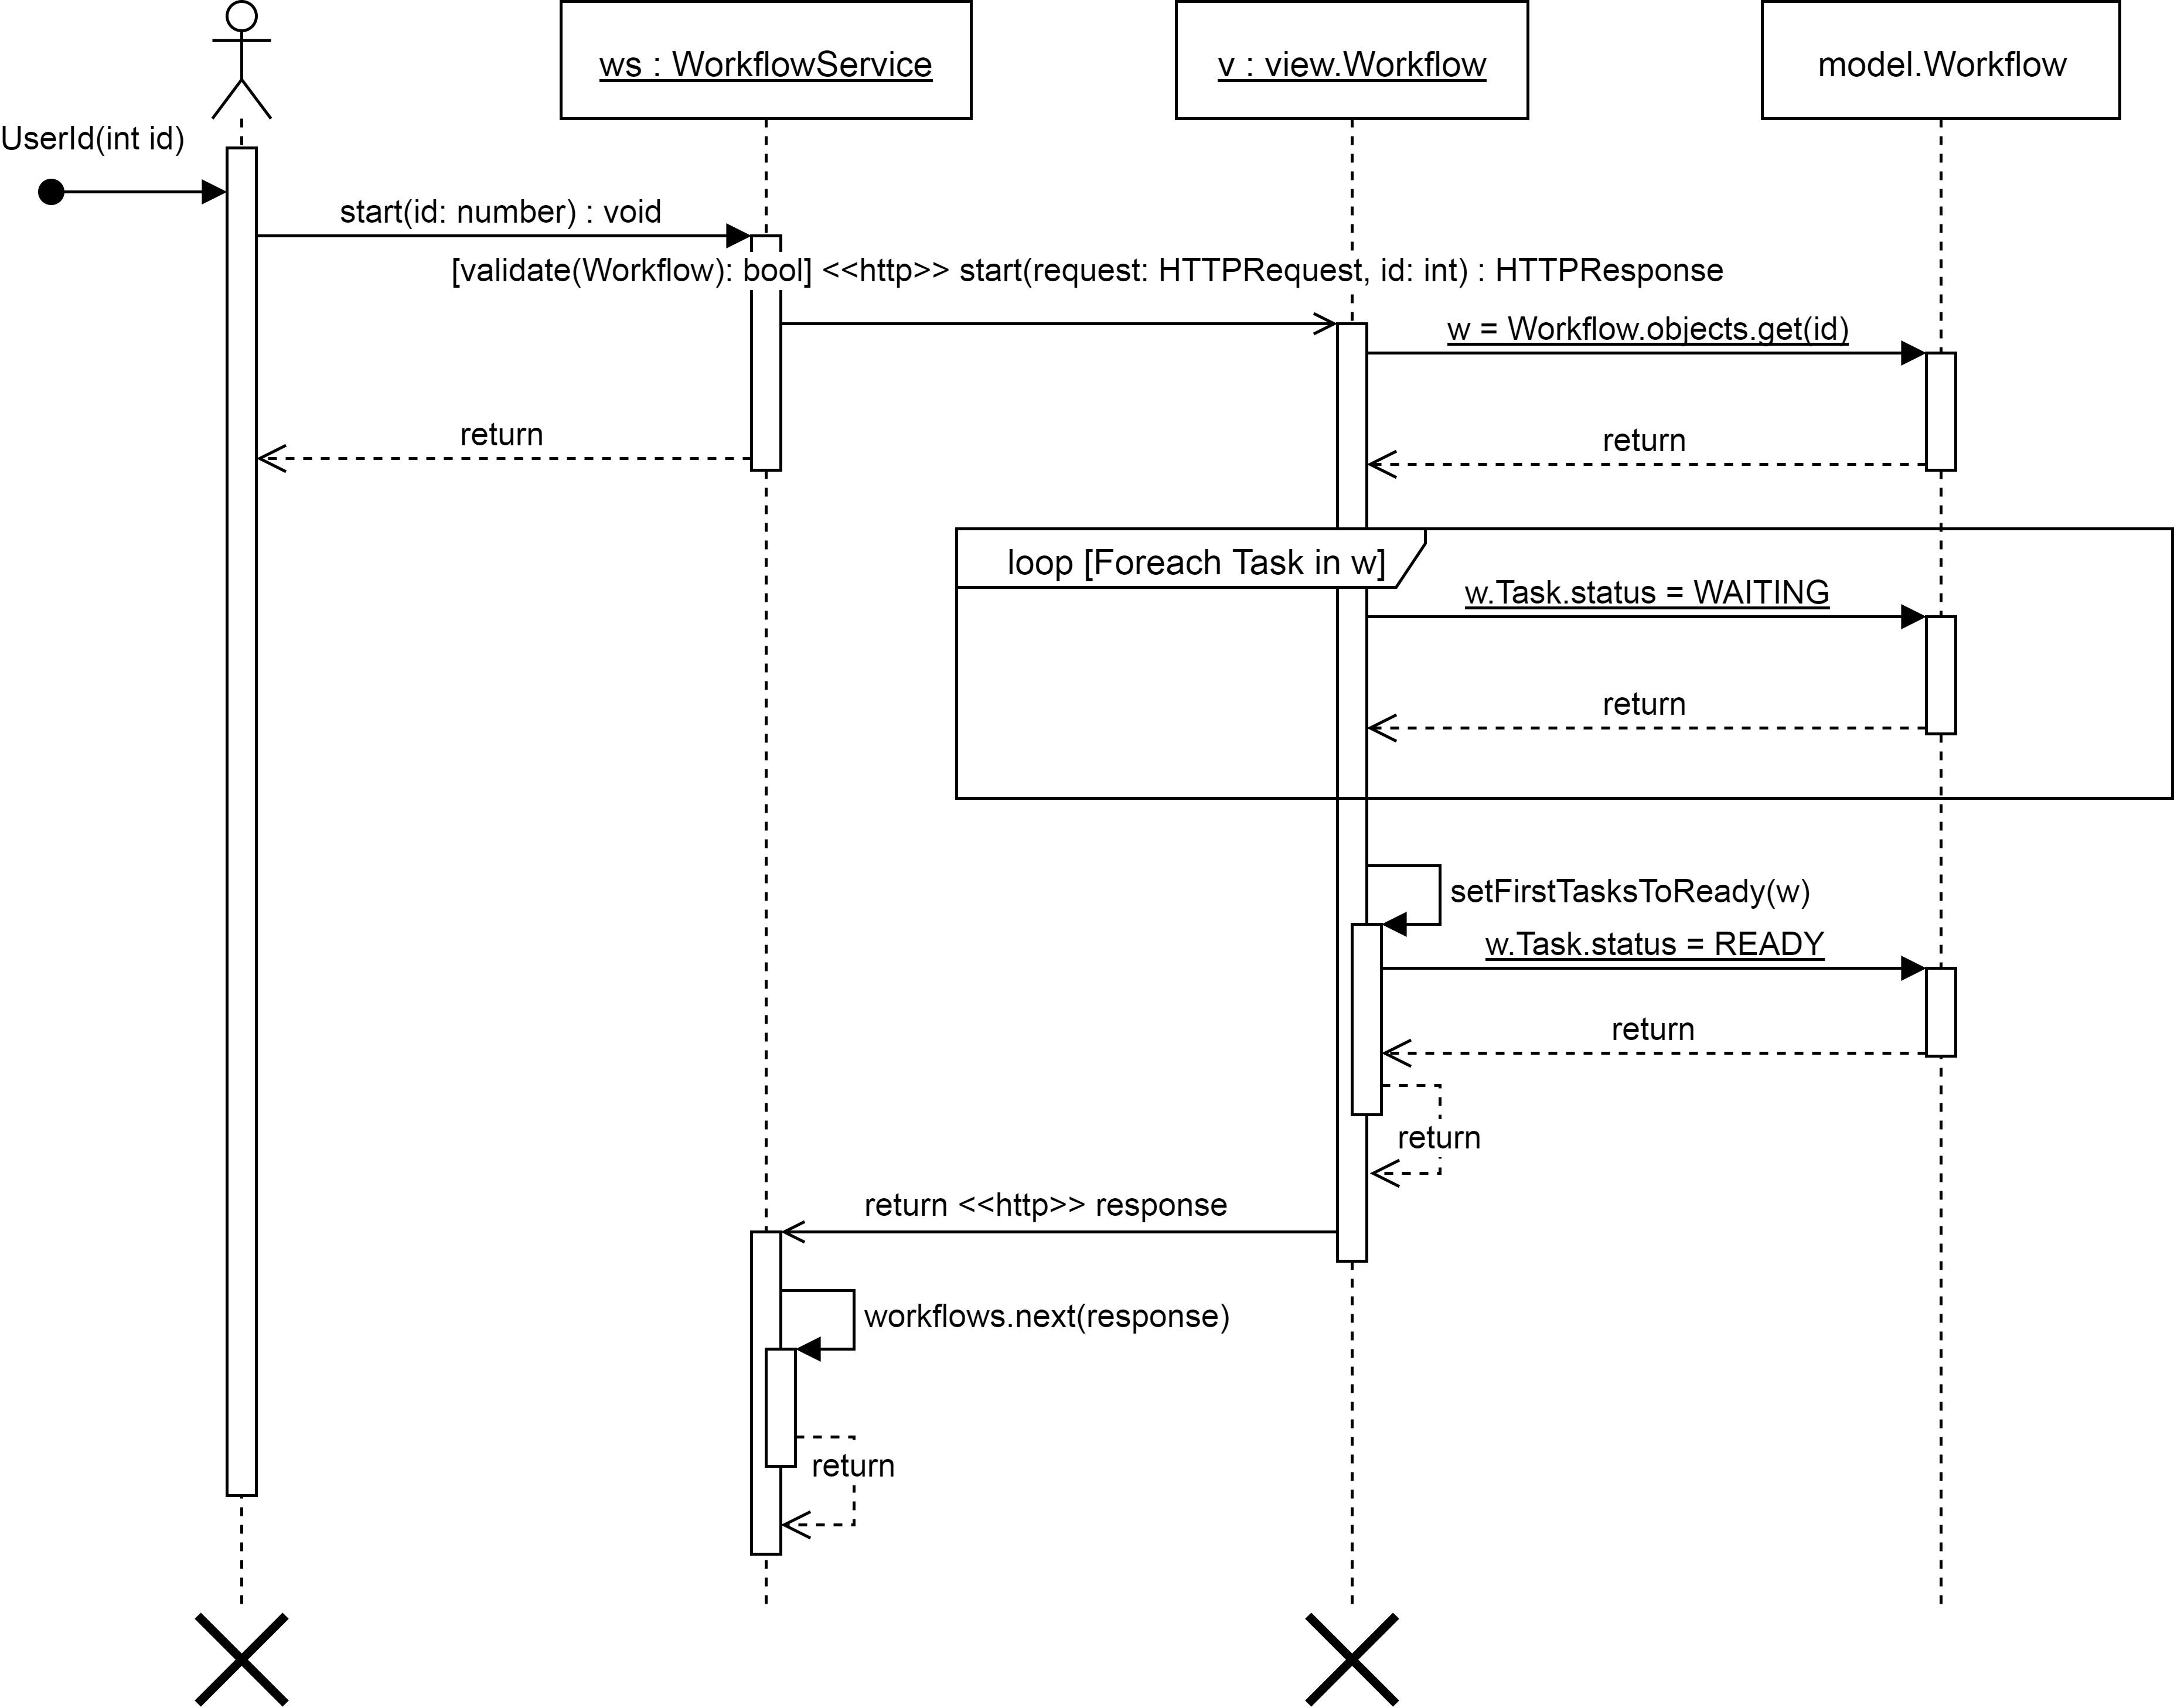
\includegraphics[width=15cm]{images/sqd_execute_workflow_client.jpg}
      \caption{caption}
      \label{fig:sqd_exec_client}
    \end{figure}
    
    \begin{figure}[h]
      \centering
      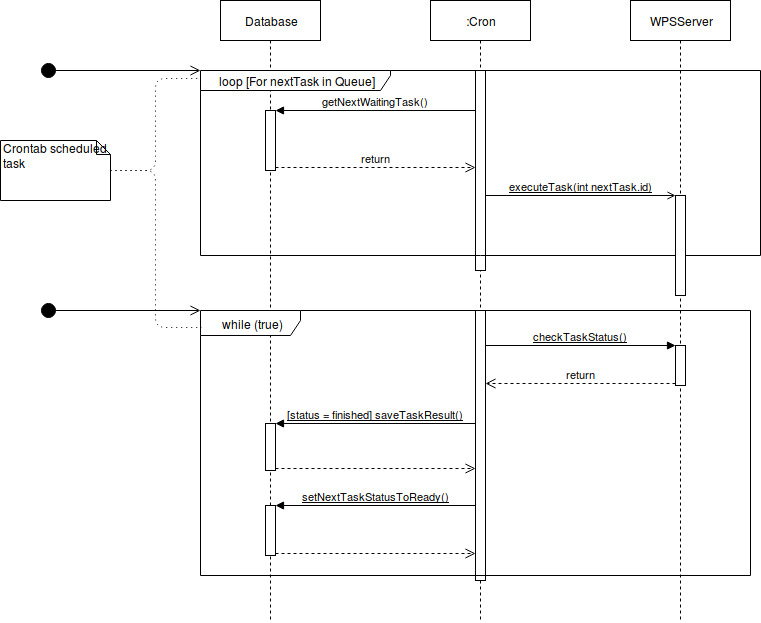
\includegraphics[width=15cm]{images/sqd_execute_workflow_cron.jpg}
      \caption{caption}
      \label{fig:sqd_exec_cron}
    \end{figure}
    
    \begin{figure}[h]
      \centering
      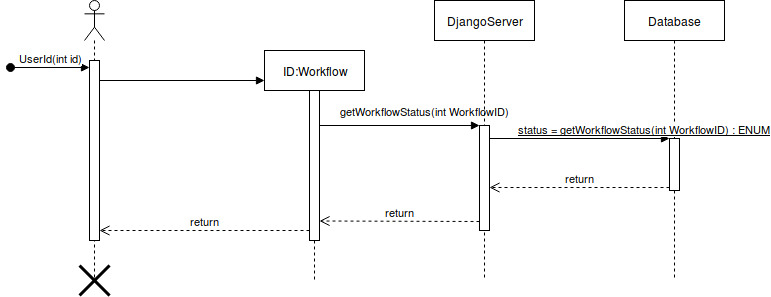
\includegraphics[width=15cm]{images/sqd_get_workflow_status.jpg}
      \caption{caption}
      \label{fig:sqd_get_wf_status}
    \end{figure}
    
    \begin{figure}[h]
      \centering
      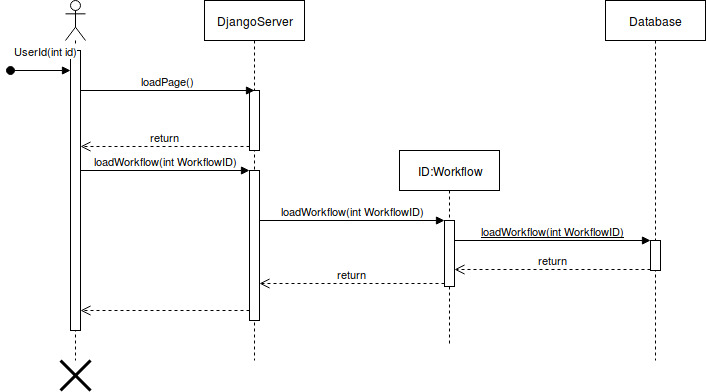
\includegraphics[width=15cm]{images/sqd_load_workflow.jpg}
      \caption{caption}
      \label{fig:sqd_load_wf}
    \end{figure}
    
    \begin{figure}[h]
      \centering
      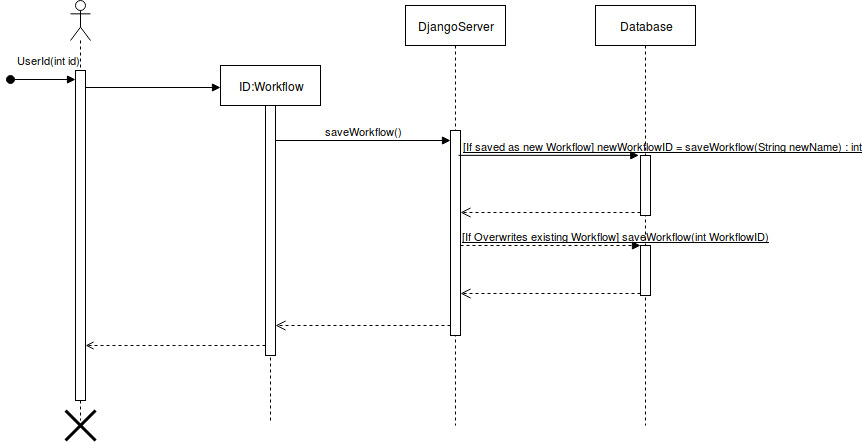
\includegraphics[width=15cm]{images/sqd_save_workflow.jpg}
      \caption{caption}
      \label{fig:sqd_save_wf}
    \end{figure}

\end{itemize}
